\documentclass[10pt]{article}
\usepackage{latexsym,amssymb,graphicx,tikz}
\usetikzlibrary{decorations.pathreplacing,calligraphy}
\addtolength{\hoffset}{-0.75in} 
\addtolength{\voffset}{-0.75in}
\addtolength{\textwidth}{1.5in} 
\addtolength{\textheight}{1.6in}

%\usepackage[dvipsnames]{xcolor}
\usepackage[colorlinks = true,
            linkcolor = black,
            urlcolor  = black,
            citecolor = black,
            linkbordercolor = {white},
            anchorcolor = black]{hyperref}
\usepackage{float}
\usepackage{fancyvrb}
\usepackage{multirow}
\usepackage{etoolbox}
\usepackage{verbatim}
\usepackage{listings}
\usepackage{amsmath}
\usepackage{bm}
\usepackage{bbm}
\usepackage{enumitem}
\usepackage{soul}
\usepackage{ulem}

\lstset{
    language=R,
    basicstyle=\ttfamily
}

\usepackage{graphicx,wrapfig,lipsum}

% === dcolumn package ===
\usepackage{dcolumn}
\newcolumntype{.}{D{.}{.}{-1}}
\newcolumntype{d}[1]{D{.}{.}{#1}}
\usepackage{multicol}

% === more new math commands
\renewcommand\r{}
\renewcommand\l{}
\newcommand\dist{\buildrel\rm d\over\sim}
\newcommand\ind{\stackrel{\rm indep.}{\sim}}
\newcommand\ud{\mathrm{d}}
\newcommand\iid{\stackrel{\rm i.i.d.}{\sim}}
\newcommand\logit{{\rm logit}}
\newcommand\cA{\mathcal{A}}
\newcommand\E{\mathbb{E}}
\newcommand\V{\mathbb{V}}
\newcommand\cJ{\mathcal{J}}
\newcommand\cN{\mathcal{N}}
\newcommand\bone{\mathbf{1}}
\newcommand\var{{\rm Var}}
\newcommand\cov{{\rm Cov}}
\newcommand\tomega{\tilde\omega}

% === spacing
\usepackage{setspace}
\onehalfspacing

\newcommand\spacingset[1]{\renewcommand{\baselinestretch}%
{#1}\small\normalsize}
% \spacingset{1.2}

% === solutions ===
% setup a new boolean
\newbool{solutionsoff}
\setbool{solutionsoff}{false}
% new environment
\newenvironment{solutions}{\color{red}}{\ignorespacesafterend}
% set conditional behaviour of environment
\ifbool{solutionsoff}{\AtBeginEnvironment{solutions}{\comment}%
\AtEndEnvironment{solutions}{\endcomment}}{}

%%%%%%%%%%%%%%%%%%%%%%%%%%%%%%%%%%%%%%%%%%%%%%%%%%%%%%%%%%%%%%%%%%%%%%%%%%%%%%

\begin{document}

\begin{center}
\begin{LARGE}DIL Data Task \end{LARGE}
\\
\bigskip
\begin{LARGE}(Senior) Research Associate \end{LARGE} 
\\
\bigskip
\begin{large}Xuting Zhou\end{large}\\
\begin{large}4/17/2024\end{large}\\
\end{center}%

\vspace{-12pt}


\section{Data Tidying}

Here’s a summary of each step undertaken to clean the data:

First,  gender information are  standardized across six variables by converting textual gender representations to numeric codes ("0" for male and "1" for female). Specific duplicates are reviewed and selectively dropped. Then, the dataset is reshaped from wide to long format, which organizes the data so each row represents a single child, while also labelling variables and values. 

Missing values for mother income and mother yob are imputed using the median income by mother's education level and calculated from mother's age, respectively. Missing child birth years are imputed based on child age.

Finally, the script checks for logical inconsistencies or errors, such as children reported to be in school at implausibly young ages or children with birth years after the survey year. Entries that don't meet logical criteria are flagged or removed (7 observations deleted).



\section{ Data Analysis}

\subsection{Summary Statistics}
\begin{center}
\begin{table}[htbp]\centering
\def\sym#1{\ifmmode^{#1}\else\(^{#1}\)\fi}
\caption{Descriptive Statistics}
\begin{tabular}{l*{1}{cccccc}}
\hline\hline
                    &\multicolumn{1}{c}{(1)}&            &            &            &            \\
                    &         All&            &            &            &            \\
\hline
Mother years of education&        9.04&        9.00&        3.53&        18.0&         1.0\\
Mother income       &      601.25&      220.00&     1694.03&     11600.0&         0.0\\
Mother age          &       33.37&       34.00&        8.65&        50.0&        17.0\\
Mother birthyear    &     1988.47&     1988.00&        8.76&      2005.0&      1972.0\\
Mother num children &        3.17&        3.00&        1.32&         6.0&         1.0\\
Child age           &        6.60&        6.00&        3.72&        13.0&         0.0\\
Child birthyear     &     2015.40&     2016.00&        3.72&      2022.0&      2009.0\\
Child sex           &        0.52&        1.00&        0.50&         1.0&         0.0\\
Child school grade  &        4.34&        4.50&        2.31&        10.0&         1.0\\
\hline
Observations        &         297&            &            &            &            \\
\hline\hline
\end{tabular}
\end{table}

\end{center}

The table provides descriptive statistics for a dataset consisting of 297 observations. The average years of education for mothers is 9 years. Mother's income shows significant variability, with an average of \$601, a median lower at \$220, and a very high SD of \$1694. The average age of mothers is 33 years, with ages ranging from 17 to 50 years. The mothers have an average of 3 children, with a range from 1 to 6 children. The data on children's school grades is available for 150 children, showing an average grade level of 4, median of 5, and grades ranging from 1 to 10.


\subsection{Balance Check}
\begin{center}
    %%% Table created in Stata by command iebaltab
%%% (https://github.com/worldbank/ietoolkit)
%%% (https://dimewiki.worldbank.org/iebaltab)
%%% The command was specified exactly like this: 
%%% iebaltab mother_educ mother_income mother_age mother_n_children child_age child_sex, grpvar(child_in_school) stats(desc(var) pair(p)) replace savecsv("C:/Users/Victoria/OneDrive/文档/GitHub/DIL_task_2024/output/raw/sum_stats.csv") savexlsx("C:/Users/Victoria/OneDrive/文档/GitHub/DIL_task_2024/output/raw/sum_stats.xlsx") savetex("C:/Users/Victoria/OneDrive/文档/GitHub/DIL_task_2024/output/raw/sum_stats.tex") texnotefile("C:/Users/Victoria/OneDrive/文档/GitHub/DIL_task_2024/output/raw/sum_stats_note.tex")

\begin{tabular}{@{\extracolsep{5pt}}lcccccc}
\\[-1.8ex]\hline \hline \\[-1.8ex]
 & \multicolumn{2}{c}{(1)}  & \multicolumn{2}{c}{(2)}  & \multicolumn{2}{c}{(1)-(2)} \\
 & \multicolumn{2}{c}{0}  & \multicolumn{2}{c}{1}  & \multicolumn{2}{c}{Pairwise t-test}  \\
Variable & N & Mean/(Var) & N & Mean/(Var) & N & P-value \\ \hline \\[-1.8ex] 
mother\_educ   & 132    & 9.129    & 165    & 8.964    & 297    & 0.690   \\
 &   & (13.151)  &   & (12.011)  &   &  \\ [1ex]
mother\_income   & 132    & 544.470    & 165    & 646.667    & 297    & 0.606   \\
 &   & (2.27e+06)  &   & (3.36e+06)  &   &  \\ [1ex]
mother\_age   & 132    & 33.106    & 165    & 33.576    & 297    & 0.643   \\
 &   & (73.439)  &   & (76.282)  &   &  \\ [1ex]
mother\_n\_children   & 132    & 3.106    & 165    & 3.218    & 297    & 0.467   \\
 &   & (1.638)  &   & (1.818)  &   &  \\ [1ex]
child\_age   & 132    & 3.795    & 165    & 8.836    & 297    & 0.000***   \\
 &   & (7.981)  &   & (7.235)  &   &  \\ [1ex]
child\_sex   & 132    & 0.492    & 165    & 0.539    & 297    & 0.423   \\
 &   & (0.252)  &   & (0.250)  &   &  \\ [1ex]
\hline \hline \\[-1.8ex]

\end{tabular}

\end{center}
The small p-value for child age in the balance test suggests significant differences in age distribution between the children who are enrolled and those who are not. This implies that age may influence or be associated with the likelihood of being enrolled in school, so it is a confounding factor.

\newpage
\subsection{Regression}
\begin{center}
    \input{Table1.txt}
\end{center}

\newpage

\subsubsection{Model Specification}
(1) Baseline Linear Regression with Robust Standard Errors: This model examines the basic relationship between a child's school enrollment and the mother's education and the child's age, using robust standard errors to account for heteroscedasticity.

(2) Baseline Logit Regression with Robust Standard Errors: It uses logistic regression to model the probability of school enrollment as a function of mother's education and child's age.

(3) Baseline Probit Regression with Robust Standard Errors: This probit regression estimates the probability of school enrollment using a normal cumulative distribution.

(4) Linear Regression with Mother Income as Control: Adds mother's income quartiles as a control variable to the linear regression, examining how economic status influences the likelihood of a child's school enrollment alongside educational and age factors.

(5) Linear Regression with Mother's Age as Control: This model controls for mother's age in addition to mother's education and child's age.

(6) Linear Regression with Number of Children as Control: By including the number of children living with the mother, this model explores whether a larger family size affects the probability of a child being enrolled in school.

(7) Linear Regression with Child's Sex as Control: Incorporates child's sex as a control to determine if there are any gender-specific differences in school enrollment rates, controlling for mother's education and child's age.

(8) Linear Regression Clustered by Village: This model accounts for clustering within villages by acknowledging potential intra-village correlation.

\subsubsection{Result Discussion}

Across all models, the coefficient for mother's education is very small and not statistically significant,  suggesting that mother's education has a minimal direct impact on whether children are enrolled in school in these models.

The coefficient for child age is consistently positive and highly significant, suggesting a strong positive relationship between child age and school enrollment. This could indicate that as children get older, they are more likely to be enrolled in school.For the linear model, it can be interpreted that with a one-year increase in child age, there is a 9\% increase in the probability of enrolling in school. For the probit and logit models, the positive sign indicates the same direction.

The coefficients for different income quartiles are small and mostly not statistically significant, indicating that income level may not be a strong predictor of school enrollment in this data.

 The R-squared values are relatively consistent across the models, around 0.456 to 0.457, indicating that approximately 45.6\% to 45.7\% of the variability in school enrollment is explained by the models. 


 \subsubsection{Graphs}
 \begin{center}
      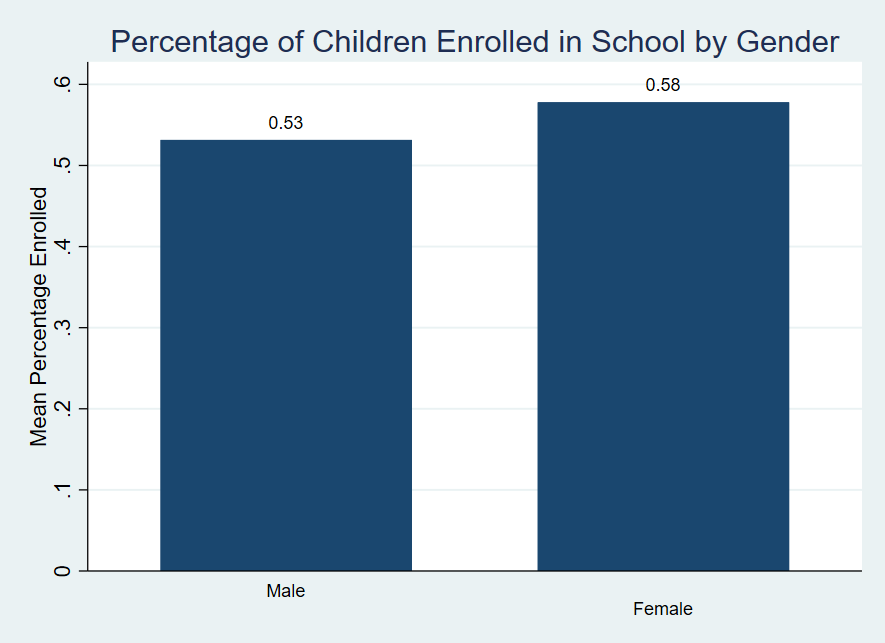
\includegraphics[scale=0.5]{school_gender_bar.png}
 \end{center}
The bar chart depicts the mean percentage of children enrolled in school, differentiated by gender. It shows that the enrollment rate is marginally higher for females (58\%) compared to males (53\%).

 \begin{center}
      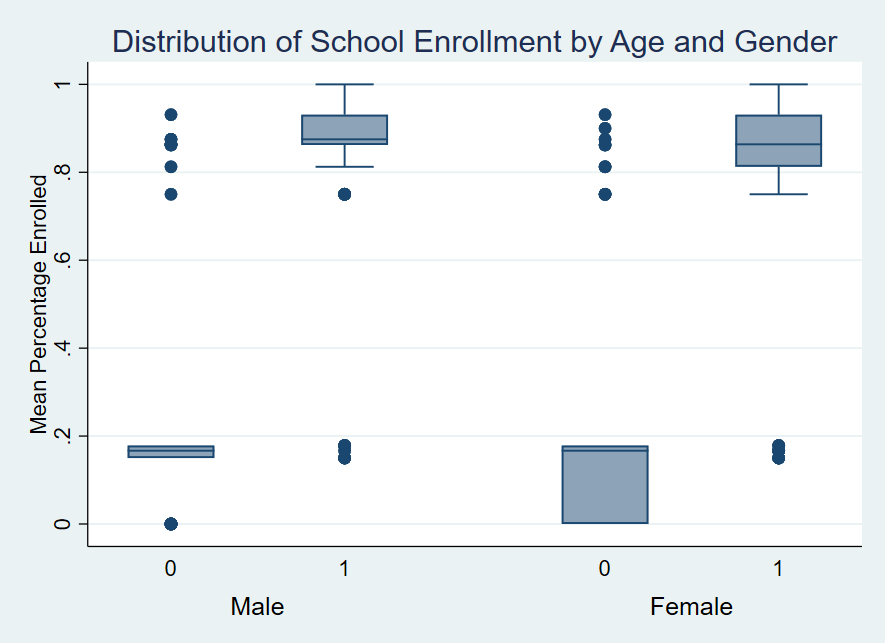
\includegraphics[scale=0.5]{school_gender_box.png}
 \end{center}

\end{document}